The introduction of an epoch breaks up the continuous timeline so that the impact of every deposit, withdrawal, and policy purchase is recorded in the specific epoch.
We can easily calculate how much is locked and how much can be withdrawn by epoch calculation.

\subsection{Locked Asset Per Share}\label{subsec:locked-asset-per-share}

The coverage of each policy locked the assets given by all underwriters by their proportion.
When a new policy is sold with the coverage of $C$, the locked asset per share is calculated as follows:

\begin{equation}
	\Delta L = \frac{C}{total\,liquidity}\label{eq:equation2}
\end{equation}

\subsection{Epoch}\label{subsec:epoch}

An epoch is a period of time during which the net $\Delta L$ is calculated and the net $\Delta L$ is the sum of the $\Delta L$ \textbf{before} this epoch minus the $\Delta L$ that has already been settled among them.

\begin{figure}[H]
	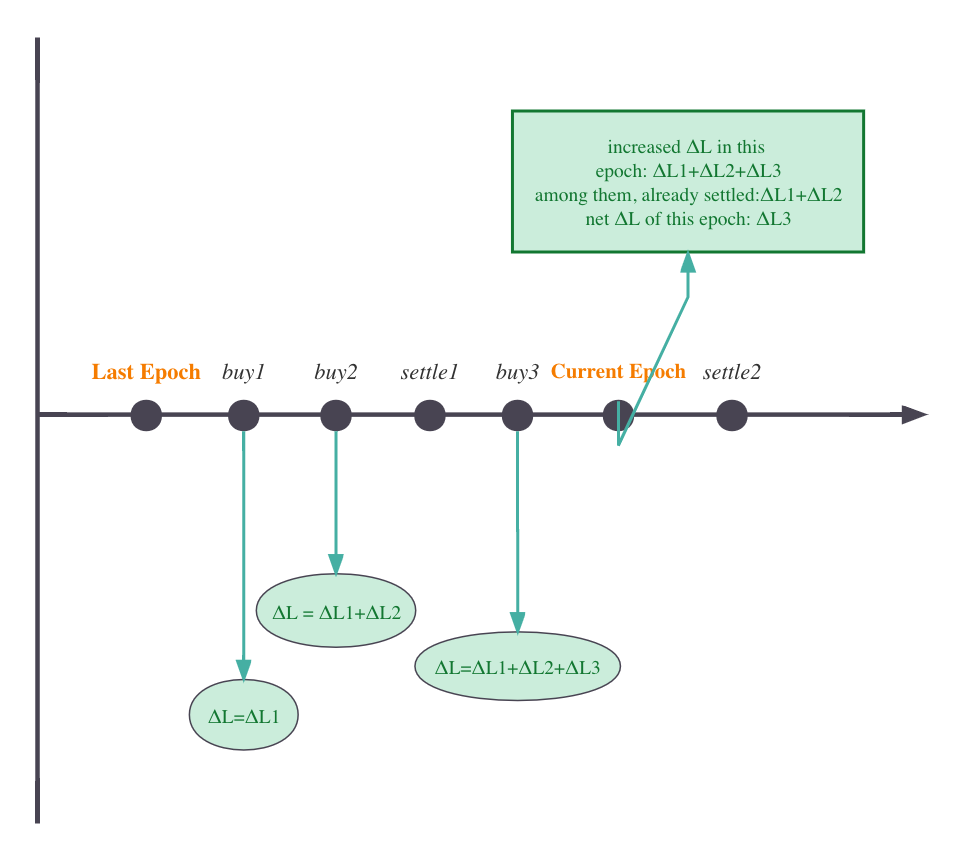
\includegraphics[width=0.8\linewidth]{net_delta_impact}
	\centering
	\caption{Epoch and Net $\Delta L$ calculation} % Figure caption
	\label{fig:epoch-and-net-delta-l} % Label for referencing with \ref{bear}
\end{figure}

The most important parameter in the epoch is the net $\Delta L$.
The epoch will also include some other parameters, such as an index and a start time.

The $\Delta L$ of a certain epoch simply indicates how much asset per share has been locked since the first epoch.
If the underwriter provide the liquidity($l$) at the epoch $i$ and exit at the epoch $j$, the locked asset($L$) can be calculated as follows:

\begin{equation}
	L = l(net \Delta L_{j} - net \Delta L_{i})\label{eq:equation3}
\end{equation}

A certain underwriter's withdrawal asset($W$) will be computed as follows:

\begin{equation}
	W = l - L  = l(1- net \Delta L_{j} + net \Delta L_{i}))\label{eq:equation4}
\end{equation}

With the equation of [\ref{eq:equation3}] and [\ref{eq:equation4}], we can easily calculate the locked asset and the withdrawal asset of each underwriter.
In this case, the underwriter can withdraw the asset at any time without a lock-up period.
